\hsection{Creating the Table}%
%
\begin{figure}%
\centering%
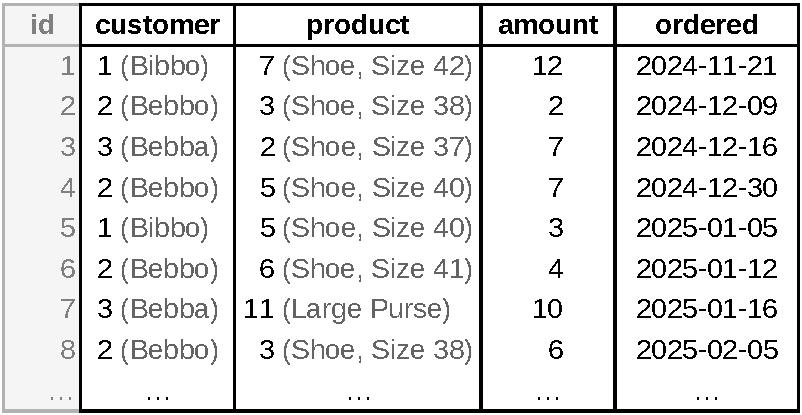
\includegraphics[width=0.72\linewidth]{\currentDir/dbStructureDemand}%
\caption{How our table~\sqlil{demand} could look like if we designed it in a spreadsheet software like \microsoftExcel\ or \libreofficeCalc. %
Since this spreadsheet would need to link its data to two other tables (for customers and products), actually implementing our factory management with a spreadsheet would become quite hard at this point.~%
(Not impossible, but very error prone and requiring serious Excel~Fu.)}%
\label{fig:dbStructureDemand}%
\end{figure}%
%
\gitLoadAndExecSQL{factory:create_table_demand}{}{factory}{create_table_demand.sql}{factory}{boss}{superboss123}%
\listingSQLandOutput{factory:create_table_demand}{%
Creating the table \textil{demand} to store the orders of our customers.%
}{}%
%
Naturally, we would like to call this table, which stores orders, something like~\sqlil{order}~(as we always use singular table names as stated in \cref{bp:tableName}).
Unfortunately, we already learned that \sqlil{ORDER}\sqlIdx{ORDER BY} is a reserved keyword in \sql.%
%
\bestPractice{neverUseKeywordsAsNames}{%
Never use \sql\ keywords or reserved words as names, e.g., for columns or tables~\cite{B2025DS:SBPASG}.%
}%
%
OK, fine, so we go with a synonym and call the table~\sqlil{demand} in \cref{lst:factory:create_table_demand}.
The structure of the table is a bit different from what we had before.
The structural sketch in \cref{fig:dbStructureDemand} indeed looks a bit odd.

But let us start slowly.
Like in the other two tables, each demand record must have a unique primary key~\sqlil{id}.
This should again be an integer number which is automatically generated by the \db\ for us.
Therefore, we define the column \sqlil{id INT GENERATED BY DEFAULT AS IDENTITY PRIMARY KEY}\sqlIdx{INT}\sqlIdx{GENERATED}\sqlIdx{BY DEFAULT}\sqlIdx{PRIMARY KEY}\sqlIdx{IDENTITY}, in the same way we already did before.

Now, however, comes something really cool:
Only customers can make orders.
Therefore, every record in the table \sqlil{demand} must be linked to exactly one record in the table \sqlil{customer}.
How can we do that?
Via so-called \emph{foreign keys}~\cite{PGDG:PD:FK}.
You see, in both of our existing tables, we have defined a \sqlilIdx{PRIMARY KEY}.
We used auto-generated integers, as we also do in the new table.
We can now define a column which also is of type \sqlilIdx{INT} and that references the primary key of another table.\footnote{%
Much later, we will formalize the concept of foreign keys in \cref{def:foreignKey}.%
}

We can write \sqlil{customer INT NOT NULL REFERENCES customer(id)}\sqlIdx{REFERENCES} to define such a file.
The name of this new column in our table \sqlil{demand} will be \sqlil{customer}.
We declare it as an \sqlilIdx{INT} which must be \sqlilIdx{NOT NULL}.
Now we write \sqlil{REFERENCES customer(id)}\sqlIdx{REFERENCES}, which basically is a constraint.
This constraint is called \emph{foreign key}.
For any value of \sqlil{customer} in our new table, makes sure that there \emph{always} is a row in table \sqlil{customer} whose \sqlil{id}~value is the same.
You cannot add a row to our table \sqlil{demand} if the \sqlil{customer} value does not match to an \sqlil{id} of one row in table~\sqlil{customer}.
You also cannot delete a record from \sqlil{customer} if its \sqlil{id} is used somewhere in table~\sqlil{demand}.
This means every single record in our table \sqlil{demand} will definitely be linked to one record in table~\sqlil{customer}.
Of course, a record in table \sqlil{customer} can be linked to many records in table~\sqlil{demand}.

Now, the customer makes a purchase.
So we want to link this purchase also to a product.
For the sake of simplicity, we only allow the customer to purchase one product at a time.
Otherwise we need yet another table {\dots} and this example will get too exhausting.
So after linking the demand records to customer records, we also need to link them to product records.
We therefore add another column that we will call \sqlil{product} by writing \sqlil{product INT NOT NULL REFERENCES product(id)}\sqlIdx{INT}\sqlIdx{NOT NULL}\sqlIdx{REFERENCES}.
As you can see, we again mark this column as foreign key by specifying a \sqlil{REFERENCES} constraint.
This time, it references the column~\sqlil{id} of table~\sqlil{product}.
In other words, every single record that we will put into the table~\sqlil{demand} will be linked to exactly one record in table~\sqlil{customer} and to exactly one record in table~\sqlil{product}.

So the customer has ordered one product.
Next we want to specify the amount of the product that the customer orders.
We create the column \sqlil{amount INT NOT NULL}\sqlIdx{INT}\sqlIdx{NOT NULL}.
For each demand, we must specify an amount~(\sqlilIdx{NOT NULL}) and that amount must be an integer, hence the~\sqlilIdx{INT}.
Having learned about constraints a while ago, we want to protect our data a bit better.
For example, we want to make sure that \sqlil{amount} is always positive, i.e., greater than zero.
Also, orders for over one million units of any product are unrealistic.
If we are about to insert a record into our \sqlil{demand} table where someone orders a million shoes, chances are that something went wrong.
So we want to define a constraint enforcing \sqlil{amount} to stay in~\intRange{1}{999\decSep999}.

We can write \sqlil{CONSTRAINT ordered_amount_ok CHECK (amount > 0)}\sqlIdx{CONSTRAINT!CHECK}.
This will create the constraint \sqlil{ordered_amount_ok} which will check that \sqlil{amount} is greater than zero.
We can also write \sqlil{CONSTRAINT ordered_amount_ok CHECK (amount < 1000000)}\sqlIdx{CONSTRAINT!CHECK}.
This would instead make sure that the ordered amount is less than one million.
We can combine both conditions into one and simply write \sqlil{CONSTRAINT ordered_amount_ok CHECK ((amount > 0) AND (amount < 1000000))}\sqlIdx{AND}\sqlIdx{CONSTRAINT!CHECK}.
Indeed, \sql\ supports logical operators such as \sqlilIdx{AND}, \sqlilIdx{OR}, and~\sqlilIdx{NOT}.
With this, we prevent any order for less than one or more than~999\decSep999 items.

Of course, we also want to store \emph{when} a customer issued the demand.
For storing dates, \sql\ offers the \sqlilIdx{DATE} type.
It allows us to specify dates in the Gregorian calendar~\cite{PGDG:PD:HU,G1582IG}.
As notation, the ISO standard format~\inQuotes{\textil{YYYY-MM-DD}}~\cite{ISO860112019} is used, where \textil{YYYY} is the four-digits of the year, \textil{MM} stands for the number month in two digits, and \textil{DD} is the day specified with two digits as well.
We then can compare dates and do all sorts of arithmetics with them.
Like the type \sqlilIdx{DECIMAL} being the canonical datatype to be used for monetary things, \sqlilIdx{DATE} is the right type for dates.
It is also a reserved word, so we cannot call our new column \sqlil{date} and we also cannot call it \sqlil{when}, as this is also reserved.
Lets use \sqlil{ordered} as name for the column storing date when the customer ordered our product.
We write \sqlil{ordered DATE NOT NULL} as column definition, because we want to enforce that it is \sqlilIdx{NOT NULL}, i.e., the order date must always be specified.%
%
\begin{sloppypar}%
Let us also insert a sanity check constraint to make sure that dates make sense.
Assume that we built our database in October~2024, then no order with a date before \textil{2024-10-01} can exist.
Furthermore, it would be unlikely that our software was still running in a thousand years, so let's also not except any date greater than or equal to \textil{3000-01-01}.
We write \sqlil{CONSTRAINT ordered_date_ok CHECK ((ordered > '2024-10-01') AND (ordered < '3000-01-01'))}\sqlIdx{CONSTRAINT!CHECK} to combine both constraints.
As you see, arithmetic comparisons have been implemented for the \sqlilIdx{DATE} datatype.%
\end{sloppypar}%
%
The table is created using the completed command in \cref{lst:factory:create_table_demand}.
In \cref{exec:factory:create_table_demand} we see the result -- there is now a new table~\sqlil{demand} in our \db.%
%
\endhsection%
%
